%----------------------------------------------------------------------------------------
%	PACKAGES AND OTHER DOCUMENT CONFIGURATIONS
%----------------------------------------------------------------------------------------
\documentclass[a4paper]{report}


\usepackage[sc]{mathpazo}
\usepackage[T1]{fontenc}
\usepackage[utf8]{inputenc}
\usepackage[english  ]{babel}
\linespread{1.05}
\usepackage{microtype}
\usepackage{xspace}

\usepackage[hang, small,labelfont=bf,up,textfont=it,up]{caption}
\usepackage[top=4cm, bottom=4cm, left=4cm, right=4cm]{geometry} 
\usepackage{booktabs}
\usepackage{float} 
\usepackage{hyperref}

\usepackage{graphicx}
\usepackage{listings}

%% Usefull for \FloatBarrier
\usepackage{placeins}

\usepackage{lettrine}
\usepackage{paralist}
\usepackage{setspace}
\usepackage{graphicx}

\usepackage{afterpage}


\usepackage{abstract}
\renewcommand{\abstractnamefont}{\normalfont\bfseries}
\renewcommand{\abstracttextfont}{\normalfont\small\itshape}

\usepackage{color}
\usepackage{xcolor}
\usepackage{titlesec}
\usepackage{inconsolata}
%% \renewcommand\thesection{\Roman{section}}
%% \renewcommand\thesubsection{\Roman{subsection}}
% \titleformat{\chapter}[hang]{\bf\huge}{}{2pc}{} 
% \titleformat{\section}[block]{\Large\vspace{0.5cm}}{}{1em}{}
% \titleformat{\subsection}[block]{\large\vspace{0.3cm}}{}{1em}{}

\setcounter{tocdepth}{1}

\newcommand\blankpage{%
    \null
    \thispagestyle{empty}%
    \addtocounter{page}{-1}%
    \newpage}

\newcommand{\ds}{\emph{DataStax\xspace}}
\newcommand{\djd}{\emph{DataStax Java Driver\xspace}}
\newcommand{\ca}{\emph{Apache Cassandra\xspace}}
\newcommand{\px}{\emph{Paxos\xspace}}
\newcommand{\jd}{\emph{Java driver\xspace}}
\newcommand{\cdt}{\emph{Cassandra Detection Tool\xspace}}
\newcommand{\dseg}{\emph{DSE Graph\xspace}}
\newcommand{\om}{\emph{Object Mapper\xspace}}
\newcommand{\sr}{\emph{speculative retries\xspace}}
\newcommand{\tp}{\emph{TinkerPop\xspace}}
\newcommand{\tdb}{\emph{TitanDB\xspace}}



\lstset{
         basicstyle=\footnotesize\ttfamily, % Standardschrift
         numbers=left,               % Ort der Zeilennummern
         numberstyle=\tiny,          % Stil der Zeilennummern
         stepnumber=2,               % Abstand zwischen den Zeilennummern
         numbersep=5pt,              % Abstand der Nummern zum Text
         tabsize=2,                  % Groesse von Tabs
         extendedchars=true,         %
         breaklines=true,            % Zeilen werden Umgebrochen
            frame=b,         
 %        keywordstyle=[1]\textbf,    % Stil der Keywords
 %        keywordstyle=[2]\textbf,    %
 %        keywordstyle=[3]\textbf,    %
 %        keywordstyle=[4]\textbf,   \sqrt{\sqrt{}} %
         stringstyle=\color{white}\ttfamily, % Farbe der String
         showspaces=false,           % Leerzeichen anzeigen ?
         showtabs=false,             % Tabs anzeigen ?
         xleftmargin=17pt,
         framexleftmargin=17pt,
         framexrightmargin=5pt,
         framexbottommargin=4pt,
         %backgroundcolor=\color{lightgray},
         showstringspaces=false      % Leerzeichen in Strings anzeigen ?        
 }
 \lstloadlanguages{
         %[Visual]Basic
         %Pascal
         %C
         %C++
         %XML
         %HTML
         %Java
         SQL
 }

\DeclareCaptionFont{white}{\color{white}}
\DeclareCaptionFormat{listing}{\colorbox{gray}{\parbox{\textwidth}{#1#2#3}}}
\captionsetup[lstlisting]{format=listing,labelfont=white,textfont=white}

\definecolor{javared}{rgb}{0.6,0,0} % for strings
\definecolor{javagreen}{rgb}{0.25,0.5,0.35} % comments
\definecolor{javapurple}{rgb}{0.5,0,0.35} % keywords
\definecolor{javadocblue}{rgb}{0.25,0.35,0.75} % javadoc
\definecolor{pgrey}{rgb}{0.46,0.45,0.48}

\lstdefinestyle{Java}{language=Java,
basicstyle=\ttfamily,
keywordstyle=\color{javapurple}\bfseries,
stringstyle=\color{javared},
commentstyle=\color{javagreen},
morecomment=[s][\color{javadocblue}]{/**}{*/},
numbers=left,
numberstyle=\tiny\color{black},
stepnumber=1,
numbersep=7pt,
tabsize=4,
showspaces=false,
showstringspaces=false,
moredelim=[is][\textcolor{pgrey}]{`}{`}
}

\lstdefinestyle{CQL}{language=SQL,
basicstyle=\ttfamily,
keywordstyle=\color{javapurple}\bfseries,
stringstyle=\color{javared},
commentstyle=\color{javagreen},
morecomment=[s][\color{javadocblue}]{/**}{*/},
numbers=left,
numberstyle=\tiny\color{black},
stepnumber=1,
numbersep=7pt,
tabsize=4,
showspaces=false,
showstringspaces=false,
moredelim=[is][\textcolor{pgrey}]{`}{`}
}

%%%%%%%%%%%%%DOCUMENT%%%%%%%%%%%%%%%

\begin{document}

\begin{titlepage}

\newcommand{\HRule}{\rule{\linewidth}{0.5mm}} % Defines a new command for the horizontal lines, change thickness here

\center % Center everything on the page
 
%----------------------------------------------------------------------------------------
%	HEADING SECTIONS
%----------------------------------------------------------------------------------------

\textsc{\LARGE University Pierre et Marie Curie}\\[1.5cm] % Name of your university/college
\textsc{\Large Internship Final Report}\\[0.5cm] % Major heading such as course name
\textsc{\large Master's degree}\\[0.5cm] % Minor heading such as course title

%----------------------------------------------------------------------------------------
%	TITLE SECTION
%----------------------------------------------------------------------------------------

\HRule \\[0.4cm]
{ \huge \bfseries Drivers and Tools at DataStax}\\[0.4cm] % Title of your document
\HRule \\[1.5cm]
 
%----------------------------------------------------------------------------------------
%	AUTHOR SECTION
%----------------------------------------------------------------------------------------

\begin{minipage}{0.4\textwidth}
\begin{flushleft} \large
\emph{Author:}\\
Kevin \textsc{Gallardo} % Your name
\end{flushleft}
\end{minipage}
~
\begin{minipage}{0.4\textwidth}
\begin{flushright} \large
\emph{Supervisors :} \\
University : Sebastien \textsc{Monnet} \\
Company : Shannon \textsc{Dennis} % Supervisor's Name
\end{flushright}
\end{minipage}\\[4cm]

%----------------------------------------------------------------------------------------
%	DATE SECTION
%----------------------------------------------------------------------------------------

{\large \today}\\[3cm] % Date, change the \today to a set date if you want to be precise


\vfill % Fill the rest of the page with whitespace

\end{titlepage}
\addtocounter{page}{-1}

\afterpage{\blankpage}

\tableofcontents
\afterpage{\blankpage}

%%%%%%%%%%%%%%%%%%%%CONTENT%%%%%%%%%%%%%%%


\chapter{Introduction}

\pagestyle{plain}
\lettrine[nindent=0em,lines=3]{T} his report describes the content of this internship made at \ds{}, UK, London. The internship was supervised by Shannon Dennis (Senior Director Engineer) and Olivier Michallat (Software Engineer) on the \ds{} side, by Sebastien Monnet (Associate Professor) and Julien Sopena (Associate Professor) on the University side.\\
\section{Summary}
I joined the Drivers and Tools Developers Team. In this report I will first make a description of \ca{}, including some additional research work on software technologies and concepts used in \ca{}. Then, I will present the first topic I've been working on, the \djd{} and enumerate the tasks I've been assigned to. I will then describe the second topic of the internship, \cdt{}. The following part will explain the last big topic of this internship, which is the DSE Graph integration in the \djd{}. I will finally conclude by explaining some miscellaneous additional work related to the 3 big topics I've been working on, and conclude.

\chapter{Apache Cassandra}
\lettrine[nindent=0em,lines=3]{A} pache Cassandra is a distributed No-SQL database created by \emph{Facebook} providing high availability and scalability, developed to handle heavy workload produced by their large amount of users and data. \ca{} has a master/slave-free architecture which allows it to provide linear scalability and helps instant recovery on hardware and software failures.\\
The purpose in the following is not to make an entire technical description of \ca{} since on the one hand, the internship doesn't involve me on the internal development of \ca{}. On the other hand, understanding the most important concepts of \ca{} is better to be able to handle correctly the interaction with an \ca{} cluster and thus, be as efficient as possible in the development of the \djd{}.

\section{General Concept}
With \ca{}, each node on a cluster of machines is responsible of a part of the data. Thus, a set of data is represented by a Partition Key, and this Partition Key indicates on which node the data will be stored, since at each node is attributed the responsibility of a range of Partition Keys. The data can (and is supposed to) be replicated among other nodes with a coefficient of replication that involves different policies of consistency and load balancing. All \ca{} nodes will then refer to these policies to manage data among all other nodes.\\
Writing on a replicated data introduce consistency challenges and is handled in \ca{} by broadcasting the \verb;write; operations on all replicas and then waiting on a quorum of replicas to confirm that changes have been applied. A default setting on an \ca{} node is to set this quorum's size to \emph{N/2} (N is the number of nodes owning a replica of the data). \verb;Reads; on replicated data can be configured according to the client's requirements. Each Cassandra node is aware of all the other nodes, and each node is responsible of the replication of the data in his range of Partition Keys.

\section{Advanced Description}
The following section will describe more precisely some of the key features that allows \ca{} to achieve its high availability and scalability characteristics. We will also make some comparison with other database systems that have different behaviors regarding these characteristics.
\subsection{Transactions}
\ca{} version 2.0 introduced a system to handle distributed transactions which, for instance allows clients using CQL operations like :
\vspace{0.7cm}
\begin{lstlisting}[label=cql-ex-1, caption=CQL Update Example, style=CQL]
UPDATE ExampleTable
SET variable = NEW_VAL
IF variable = OLD_VAL;
\end{lstlisting}
\vspace{0.7cm}
This \emph{IF} condition may not be a big constraint when developing a relational database, but with a fully distributed database, this precondition causes several complications : 
\begin{itemize}
	\item How to achieve linearizability and consistency with distributed transactions ? Use Consensus.
	\item How to keep an acceptable throughput with a Consensus algorithm ? \px{}\cite{Lamport1}.
\end{itemize}
{\bfseries But}, building these types of transactions involved the need to add some extra-phases to the original \px{} algorithm. Here we won't recall \px{}'s proofs that define the Consensus guaranties when a majority of nodes responds positively in the \emph{Accept} phase. But original \px{} algorithm allows to agree on one value that won't be changed, besides that, what we want to do in \ca{} is to achieve linearizibility on a suite of operations (or we can say 'values'). Nodes would then be sure of the consistency of the data since every node would have executed operations on its replica in the same order. \\
To do so, a node must find a way to 'restart' the algorithm in order to make a new decision on another value and chain the algorithm executions. First way to do that would be to build a distributed edit log file based on successive Consensuses made with \px{} (a brief review of \emph{Google}'s solution to do that later). To chain \px{} execution in \ca{} the idea has been to add an extra phase to the algorithm called \emph{commit} phase which simply sends \emph{commit} messages to all nodes to notify them the end of the algorithm.\\
Another point about using \px{} algorithm in our context is that our need is to execute a \emph{compare-and-set-like} operation, whereas \px{} algorithm allows to only \emph{set} a value without making the comparison. \\
Making this possible implied adding another extra-phase to the original \px{} algorithm, which is, after receiving a majority of responses from the \emph{prepare} phase. The newly decided coordinator will send a request to all nodes to get their local value of the replica. If the expected value match, the node proceeds to the following of the algorithm (\emph{accept}), if not, the algorithm stops and the value is not updated.
With these solutions, \ca{} simply implements \emph{compare-and-set} distributed operations on multiple variables sequentially with the guaranties of the \px{} algorithm. With the cost of the overhead produced by the 2 extra-phases.

\subsubsection{\emph{Google}'s distributed edit log file}
\emph{Google}'s approach to build a distributed fault-tolerant database based on \px{} was described in their paper \emph{Paxos Made Live}. It actually explains that even if \px{} algorithm could be easily described in one page of algorithmic instructions, engineering a production-ready software based on it, is not so simple.\\
Indeed, to be fault-tolerant an application has to rely on the hypothesis that a machine doesn't have unlimited memory, and that it can suffer of hard disk failures. Also, the implementation has to be adaptable to different hardware infrastructures since real systems are rarely specified precisely.\\
The approach taken here was to build a \emph{fault-tolerant} log file that will be describe the operations to be applied on a replica of data. All the replicas hosts would then agree with \px{}'s Consensus on the content of this log file and each one would keep locally a version of it. Building a file log of sequential operations implies to chain \px{} executions, which are called \emph{instances} (the same idea described earlier for \ca{}).\\
In order to increase throughput and performance of the \emph{instances}, two additional concepts came up in the paper : 
\begin{itemize}
	\item When a coordinator sends data in an \emph{Accept} message, it can concern not only one variable, and update multiple set of variables. So when the \emph{Accept} message is acknowledged by a majority of nodes, all the values will be modified at the same time.
	\item To avoid as much \emph{Propose} messages overhead as possible, the algorithm could state that a coordinator, once it has passed the \emph{Accept} phase with his value on a previous instance, can stay \emph{elected} for certain period of time. And thus, it can chain \emph{Accept} phases for as long as he is coordinator. He is then called \emph{master}. After that, when a node starts a new instance of \px{} algorithm, it first tries to grant a lease from the coordinator (\emph{master}) of the last instance and sets it as his coordinator for this new instance.
\end{itemize}
\emph{Master} leases doesn't corrupt the \px{} algorithm since a \emph{master} is elected it can fail, and after a certain period of time (\emph{heartbeats}), a new instance will be run and will elect a new \emph{master}.\\
Besides that, \emph{master leases} improve performance with the fact that when a \emph{master} is elected by a majority of replicas, the \emph{compare} of a \emph{compare-and-set} operation on a \emph{master} can be done locally since once it knows that it has been elected, the \emph{master} knows no other node is going to acknowledge \emph{Propose} messages from another coordinator. Each time a \px{} instance is ran, replicas \emph{grant} a lease from the \emph{master} of the previous instance. For \emph{Google}, this implementation of \px{} was used as backend of \emph{Chubby}, a \emph{fault-tolerant master-slave} distributed locking system which during its computation stores \emph{Chubby} lock files in a distributed database with replication, and that was then, using this implementation of \px{}. This way, \emph{Chubby masters} and \emph{Paxos masters} could be correlated to improve throughput of the application.\\
Since the log file concerns actions to be applied on a certain data structure, the data structure's history has to be saved, so as for the log file, in case of when a replica fails and has to recover. To handle limited memory restrictions, persistent state's history has been achieved by making \emph{snapshots}. With a proper \emph{snapshot} algorithm the data could be saved in a period of time related to the memory capacity and the \\
log file can also be truncated since it only needs to contain the operations executed since the last \emph{snapshot}.\\
Implementing these concepts and other technical details allowed to build distributed fault tolerant database relying on \px{}.

\subsection{\ca{} local persistence} % (fold)
\label{sub:ca_local_persitency}

To achieve local persistence of writes on data in the most efficient way, \ca{} rely on some principles that helps acquiring better performance and safety.\\
Each write operation involves a new entry in a local commit file. The write in this file is persisted and it is assumed in \emph{Facebook}'s paper on \emph{Cassandra} that this commit file is stored on a dedicated hard disk used only for this purpose, to maximize throughput in regard of the sequential constraints of this one.\\
To optimize response time on a \emph{read} request, \ca{} first does a lookup in the in-memory data structure of most recent data, and if not present, do a lookup on persistent storage. Data is stored in many files on a disk, (ordered from newest to oldest) each part of the data represented by a key. To prevent browsing files that do not contain the needed key, each file owns an index which describes all the keys the file is composed of. This index is called \emph{bloom filter}.

% subsection ca_local_persitency (end)

\subsection{Gossip membership protocol and possible ATTACKS} % (fold)
\label{sub:gossip_membership_protocol_and_potential_weaknesses}

With \ca{}, since the data is distributed and replicated, each node maintains locally the situation it is aware of each other node in the \emph{ring} (the \emph{ring} represents the nodes organized according the distribution of the tokens). \\
To maintain a coherent distribution of the tokens, in case of when a node fails, a membership protocol called \emph{Gossip protocol} runs regularly to keep the ring coherent. In short, this this protocol consists of : an \emph{initiator} node starting a \emph{gossip} round by sending a \emph{receiver} node his current view of all the nodes. The \emph{receiver} updates his view according to the initiator's view (assuming that there's a additional technical process that can insure that a view is more recent than another). And if the view also needs to be updated on the \emph{initiator}, the \emph{receiver} sends the updates in an \emph{ack} message. The \emph{initiator} then updates his views and acknowledges them to the \emph{receiver}.\\
After explaining that this protocol brings a great benefit to the consistency of the system, we will see that some experiences proved that in some cases it can also become a weakness...\\
This\cite{Aniello13} paper explains the vulnerabilities to such a protocol, stating that, in the \emph{gossip} protocol, there is no concern about the about what could happen if the information in these \emph{gossip} messages are false, corrupted. With this statement, we can imagine 2 types of of attacks involving a byzantine node that's purpose is to send wrong information among the network.\\
A first \emph{attack} would be to make some nodes (even maybe all) believe that a node is \emph{down} while he is not. Sending a message to a \emph{receiver} node, falsely up-to-date, saying that a node is \emph{down} can lead the \emph{receiver} node to update his view with a wrong information. The second \emph{attack} is the opposite of the first one, a byzantine node waits for a node to fail, and while the node is failed, the byzantine one sends \emph{gossip} messages to every other saying that for it (the last updated view) the node is still up.\\
This kind of \emph{attacks} can have a big impact on the performance of the database when there's big loads of data to handle. \\
It could in the first case, contradict load balancing policies by lowering the usage of the \emph{faked} node, in the second case, involve a great number of lost requests. The paper reports a percentage of up to ~83\% of lost requests when disseminating up to 75\% byzantine nodes in the network, using the \emph{ALL} consistency level. It also describes a \emph{relatively low} performance impact solution to the excess of trust in the \emph{gossip} protocol. It consists in adding an encryption layer to the protocol, allowing to insure that information provided is not from a byzantine node. A little bit like Byzantine \px{}\cite{Martin}, with the cost of encryption.

% subsection gossip_membership_protocol_and_potential_weaknesses (end)

\chapter{Java Driver for Apache Cassandra}
\lettrine[nindent=0em,lines=3]{T} he first and main topic of this internship have been to contribute to the open-source project \djd{}. Thus, I will describe how the \djd{} represents more than a simple software that sends packets to a server, by explaining some of its most important and useful characteristics. I will after expose some notable features I've been helping adding in the driver, then present the features I have been working on by myself.
\section{Introduction}
The \djd{} is a high level library that handle interaction with a \ca{} database. The \djd{}'s main goal is to successfully establish connection to a node, send requests and receive results. It is closely tied to the \emph{Cassandra Query Language} and communicates with \ca{} using a communication protocol named \emph{Native Protocol}.

\section{Basic concepts}

\subsection{Connection}
The first step, to successfully achieve communication with a \ca{} database is to be able to successfully connect to it through the network. With the \djd{}, it is possible to connect to any of all the nodes in the Cassandra cluster by providing at least one IP address of one node.\\
The main representation of the connection to a \ca{} cluster is exposed through a \verb;Cluster; object. To optimize latency, throughput and scalability (more on that later), the driver will then gather a lot of information from the node it is connected to. The first node connected, becomes what we call the \emph{Control connection}. After connecting to the first node, the driver will execute several additional tasks :
\begin{itemize}
   \item Connect to all other known up nodes in the cluster.
   \item Collect cluster metadata.
   \item Collect schema metadata.
\end{itemize}

After these tasks successfully executed, a \verb;Session; object is returned to the client. This \verb;Session; object is the object from which the client will be able to send, prepare, and bind \emph{CQL} statements.

\subsection{CQL}
The \emph{CQL} query language is a database query language specific to \ca{}. Its purpose is to fit the most possible to the existing universal \emph{SQL} query language, and in the same time provide \ca{} specific syntax. \emph{CQL} is then designed to provide options and tools to handle distributed datasets, with the possibility to manage consistency levels, replication factors, data partitioning, node management, and so on. \emph{CQL} statements are sent by the driver to a \ca{} cluster through the \emph{Native protocol}.

\subsection{Native protocol}
The \emph{Native protocol} is a network applicative protocol built on top of \emph{TCP}. It has been designed to be fully asynchronous, hence, on the driver side it allows to accumulate queries on a single connection in an asynchronous manner. Indeed, each request on a connection gets assigned to a request identifier, named stream id, created in a thread-safe way on the client side. Multiple requests can be sent asynchronously and concurrently through the connection, each response coming back will be assigned to the stream id it has been issued from. The driver also adds a client-side timestamp on each request, to insure order of requests when needed by the user.
\emph{Native protocol} also allows security functionalities like server-side authentication and SSL encryption.\\
Most of the work accomplished by the \djd{} is to encode and decode data sent and received through the \emph{Native Protocol}.

\subsection{Processing responses}
The \emph{Native protocol} being fully asynchronous, a client has the possibility the process the results of its queries either synchronously or asynchronously. Internally, everything is handled asynchronously, every request implies the creation of a \verb;Future; object from the Java's \verb;Future; library. On these \verb;Future; objects we can define callbacks to fill the data when a connection notifies that the data has arrived through the connection. Since internal processing in the driver is asynchronous, most part of the code is thread-safe.

\subsection{Metadata}
Aside from sending statements, and processing results, the \djd{} exposes a complete description of the cluster, schemas, tables, indexes, partitions, through the \verb;Metadata;. This metadata is computed at the \verb;Cluster;'s initialization and is maintained up-to-date all along the \verb;Cluster; object life span. Having this metadata improves the driver knowledge of the current status of the system, and allows the driver to adapt it's behavior according to it. The metadata is also exposed to clients through API specific objects.



\section{Advanced Features}
In this part I will try to explain some more advanced features that contribute in making the \djd{} more powerful, scalable, tunable, and probably jusifies the 70.000+ public downloads of the software each month. I will present some of these features in details because we'll see later that some of my assignments for the internship were to maintain, or improve those features, and acquiring a strong understanding of these notions have also been the first step of the internship. It is also important to avoid altering the behavior of such functionalities when developing new features.

\subsection{Connection Pooling}
As stated earlier, at cluster's initialization, the driver establishes connection to the first IP address that has been specified, and this node becomes for the driver, the \emph{Control connection}. In addition to that, the driver will also establish a connection to all the other nodes in the cluster. This is made for multiple purposes. First, in case of a clear failure on a node, which doesn't respond in time (timeout), or returns an internal exception, so the driver still has a way to process the request for the client. Remember that \ca{}'s architecture is Master-less, which means every node is able to handle every request, the nodes are aware of the data repartition (Token routing) and replication. The second advantage of connecting to all nodes is load balancing. Indeed, to handle heavy loads needed for some applications, the driver is able to distribute the requests to all nodes equally, so that one node connected doesn't get overloaded (more information in the \emph{Policies} section).\\
But that's not all, to achieve even better throughput the driver establishes pools of connections for each host. This is needed mainly because requests can take a viariable amount of time to be executed on the server side, and since everything is asynchronous, the protocol accepts adding pending requests on a same connection (thanks to stream ids). But it has its limits, the \emph{Native protocol} version 2 can only handle a maximum of 128 simultaneous requests on a same connection. This limit can quickly transform into a bottleneck, that prevents achieving high throughput. That is why the driver has pools of multiple connections for each node.\\
Unfortunately achieving high throughput comes with the price of having to tune and maintain the connection pools. Thanks to the highly tunable nature of the driver, users are able to define rules to dynamically resize connection pools according to the current load. Indeed when the load becomes more consequent, the driver automatically increases the number of connections in the pools. We can detect that the load becomes heavier because the driver maintains a number of pending requests per each connection. Hence, the decision to open a new connection is made when all existing, except one, connections in the pools have the maximum allowed pending requests, and when the number of pending requests on the last connection becomes higher than a defined \verb;threshold;.\\
The driver provides the option to set the original number of connection per pool, the maximum number of connections to create, and set the \verb;threshold; to use for connection creation, and also set the \verb;threshold; indicating whether to close a un-needed connection.\\
With fine tuning of these parameters, our experiments prove that the driver have been able to issue comfortably peaks of 100k requests/node.\\
In more recent versions of \ca{}, the \emph{Native protocol} have been updated and is now able to support 32768 requests on each connection. This greatly helps improving the usage of a connection pool, unfortunately experiments still show a bottleneck in using a limited number of connections in pools, more on that later, in the \emph{Netty} section.

\subsection{Policies}
The Java driver is highly tunable, and some of its most important settings are defined with policies. A policy is a Java object defined by the user, implementing an \verb;Interface; of the driver, and whose methods will be injected in the driver's code. The user can specify the policies during the cluster's creation.

\subsubsection{Load Balancing Policy}
The driver provides a set of pre-configured and highly tested load balancing policies. However, a user can injects its own. The load balancing policy is the class defining the \verb;queryPlan;. The \verb;queryPlan; is the object which defines what will be the host chosen to send each query, it's a Java \verb;Iterator; which will return a host each time the driver needs to send a request. This setting is important in order to distribute the load on as much nodes as possible and thus, avoid bottlenecks and improve throughput.\\
For example, the most common and meaningful balancing policies to use, for normal use-cases is the \verb;TokenAwarePolicy; with a \verb;DCAwareRoundRobinPolicy; fallback option. 
It is set constructing the following object a cluster's creation :
\begin{lstlisting}[label=lbp-ex-1, caption=Creation of the cluster, language=Java]
Cluster.builder()
   .withLoadBalancingPolicy(new TokenAwarePolicy(new DCAwareRoundRobinPolicy, true));
\end{lstlisting}
This setting allows to send statements to directly to hosts having a local replica of the data according to the routing key of the statement (that's the goal of the \verb;TokenAwarePolicy;) and if no local replica was found, send the statement in a round-robin fashion, to hosts from the same DataCenter (the role of the \verb;DCAwareRoundRobinPolicy;).\\
Other useful Load balancing implementation are provided from the driver such as \verb;WhiteListPolicy;, or \verb;LatencyAwarePolicy;. But users can still implement their own policy and inject it in the driver. By default the driver uses a \verb;RoundRobinPolicy; based on its knowledge of the hosts located in Cassandra's table \emph{system.peers}.

\subsubsection{Retry policy}
The retry policy defines what should be the behavior of the driver in case a query sent to a Cassandra node happens to fail, and the node originally contacted for the request sends back to the driver the error corresponding.\\
Executing a query can fail in two ways : 
\begin{itemize}
   \item The error happens on the driver side. The driver is not able to communicate to the server in the required time, or no host is available anymore, a network failure occurs.
   \item The coordinator (host contacted for the query) is reachable for the driver, and the coordinator receives the query, but an issue internal to the processing on the server-side occurs. This can be a consistency level issue, a network issue between multiple Cassandra nodes, and so on.
\end{itemize}
For the first case, the driver provides an API to tune the socket options. With this, users can set timeouts, buffer sizes, etc.
The second point is handled differently, when a server-side issue occurs, the coordinator will be able to send an error message to the driver. Then, the reaction of the driver according to different kind of errors will be defined by a \verb;RetryPolicy;.
The errors returned can be of 3 types : 
\begin{itemize}
   \item Read timeout
   \item Write timeout
   \item Unavailable host
\end{itemize}
Each of these errors is likely to happen because the consistency level required for the query could not be met (e.g if 3 replicas were required but only 2 responded within the defined server-side timeout). Then, the driver will call the corresponding method in the \verb;RetryPolicy; object it has been constructed with. If the error is a \verb;ReadTimeoutException;, the driver will call \verb;Retrypolicy.onReadTimeoutException();.\\
As usual, the driver provides highly tested and pre-configured Retry policies. An interesting one is the \verb;DowngradingConsistencyRetryPolicy;. Thanks to this policy, we can define that when a \verb;ReadTimeoutException; happens, the driver will re-send the request, to the same host, with a consistency level reduced by 1 and only once, otherwise a Java exception is thrown.

\subsubsection{Reconnection policy}
A reconnection policy is meant to be used in cases where a connection in a pool gets closed because of a particular error. The reconnection policy mainly helps define the time before the next reconnection attempt gets scheduled. Users can explicitly set this time, or \verb;ConstantReconnectionPolicy; can help define a constant time before reconnection, and \verb;ExponentialReconnectionPolicy; helps define a base delay which will grow exponentially, until a maximum delay is reached, then when the maximum is reached, it will stay constant.

\subsection{Object Mapper}
The \om{} is an additional module of the driver, distributed as a separate Maven artifact. This module provides a simple object mapping that avoids most of the boilerplate of converting CQL results to and from a Java object. It handles basic CRUD operations in Cassandra tables containing UDTs, collections and all native CQL types.\\
The object mapper is configured through annotations. The \om{} can map all native \emph{CQL} types and also collections, user defined types. The following is an example of its usage : 

\begin{lstlisting}[label=om-ex-1, caption=Object Mapper example, style=Java]
`@UDT(keyspace = "ks", name = "address")`
class Address {
    private String street;
    `@Field(name = "zip_code")`
    private int zipCode;
    // ... constructors / getters / setters
}

`@Table(keyspace = "ks", name = "companies",
       readConsistency = "QUORUM",
       writeConsistency = "QUORUM",
       caseSensitiveKeyspace = false,
       caseSensitiveTable = false)`
public static class Company {
    `@PartitionKey`
    `@Column(name = "company_id")`
    private UUID companyId;
    private String name;
    private Map<String, Address> aMap;

    // ... constructors / getters / setters
}
...

/* Application code */
Mapper<Company> mapper = manager.mapper(Company.class);

UUID companyId = ...;

Map<String, Address> map = 
                     new HashMap<String, Address>();
map.put("office1", new Address("street1", 01000));

Company c = 
        new Company(companyId, "GreatestCompany", map);

mapper.save(u); //The mapper persists the object
\end{lstlisting}
The mapper also provides accessors, and has its set of \emph{Option}s for tuning.

\subsection{Query builder}
The query builder is another module of the driver, that comes packaged with the driver core component. As its name states, the query builder helps creating valid \emph{CQL} queries in an object oriented fashion. It handles most of the possibilities offered by the \emph{CQL} syntax.\\
Here's a quick example : 
\begin{lstlisting}[label=qb-ex-1, caption=Query Builder example, style=Java]
QueryBuilder builder = new QueryBuilder(cluster);
Statement select = builder.select().all().from("foo").where(gt("k=1 OR k", 42)).limit(42);
// Result is : "SELECT * FROM foo WHERE \"k=1 OR k\">42 LIMIT 42;"
\end{lstlisting}
\newpage


\section{Notable new features}
The previously presented features compose the core functionality of the driver. However, since the beginning of this internship, some other interesting features have been added, on which I was not directly in charge but I've been helping, reviewing and contributing.

\subsection{Speculative retries}
\emph{Speculative retries} is a way to improve a query execution in case a host happens to be long to respond, because of a GC pause, for example. Where \sr{} acts, is that the driver will automatically, transparently for the user, send the statement to another host in case it responds faster.\\
In case speculative retries are fired, the previously sent statements are canceled on the hosts.\\
\begin{figure}[ht!]
\centering
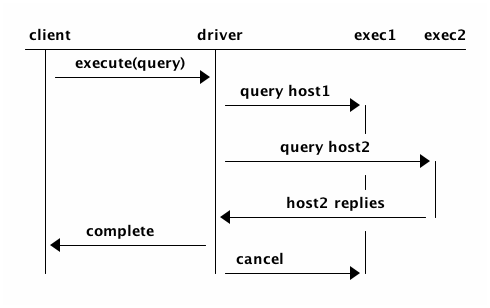
\includegraphics[scale=0.7]{spec_rec.png}
\caption{How speculative retries work}
\end{figure}
With \sr{} comes the question to know when a statement is idempotent or not. Indeed, in \ca{} a statement is not idempotent when it : 
\begin{itemize}
   \item updates a \verb;counter;\footnote{A counter is a special column type in \ca{} that's optimized and tunable in consistency and cache options on the server side. A counter can only be incremented or decremented by reading the current value and applying a \emph{delta}. Thus, the nature of this type is non-idempotent.} ;
   \item adds an element in a collection like a \verb;list; ;
   \item uses non idempotent \emph{CQL} functions like \verb;now();.
\end{itemize}
Hence, since the driver does not parse text \emph{CQL} statements that it sends to the server, a conservative approach has been taken and all statements are considered as non-idempotent by default. Users have to explicitly indicate that the statement is idempotent through a statement's \emph{option}. The only moment when the driver can know if a statement is idempotent, is when the query is constructed with the \emph{Query Builder}.\\
\emph{Speculative retries} are configurable on the delay new retries are scheduled. This delay is compatible with another driver component, the \emph{Latency Tracker}.\\
Indeed, the driver implemented its own \emph{Latency Tracker}, added to track each hosts' latencies the driver observes during its life-cycle. Then, the driver can process this information and adapt its behavior. The driver also offers a \verb;PerHostPercentileTracker; which, thanks to the \emph{HdrHistogram} library, allows building statistics on top of the latencies observed and provide percentile-based previsions for each hosts.

\subsection{Query Logger}
Recent versions of the driver comes with a new \emph{Query Logger} module. It is then possible to follow the execution of all queries and determine whether queries take more time than other ones. Users can configure the driver to log messages when queries either :
\begin{itemize}
   \item get successfully executed within a configured threshold ;
   \item take longer than a configured threshold ;
   \item return exceptions or fail.
\end{itemize}
The threshold mentioned above can be a constant value, declared at \verb;Cluster;'s initialization. Or, for a more advanced usage, the threshold can be dynamic, and paired with the \verb;PerHostPercentileTracker;. That way, users can easily detect a sudden latency happening on the network, maybe due to congestion, router failures, etc.
\begin{lstlisting}[label=ql-ex-1, caption=Query Logger live action, style=Java]
TRACE [cluster1] [/127.0.0.1:9042] Query too slow, took 329 ms: SELECT * FROM users WHERE user_id=? [user_id=42];
\end{lstlisting}

\subsection{Netty}
On the one hand, the \djd{} have been using \emph{Netty} since its first versions, on the other hand on recent versions of the driver we have decided to update \emph{Netty} to a major new version (\emph{Netty 4}) and that implied important conception and code changes in the driver. So, I will briefly in this section describe how \emph{Netty} works, and then introduce the biggest and most interesting changes using \emph{Netty 4} implied on the driver.

\subsubsection{Brief description (at least I tried, to be brief)}
Basically \emph{Netty} is a very well known and well renowned Java network I/O framework, designed to  tackle heavy loads, be scalable, and drastically be easier to use than Java OIO and Java NIO\footnote{Java Old I/O and Java New I/O, the former is the first developed blocking Input/Output Java API based on sockets streams, the latter being the non-blocking one introduced first in JDK 1.4, then upgraded and named NIO.2 starting from JDK 1.7, buffer-oriented.} libraries. It is used on some of the most scalable and powerful actual industry platforms\footnote{Facebook, Twitter, Instagram, Netflix, Spotify, Apple, the list is quite long... http://netty.io/wiki/adopters.html}, and is the subject of many presentations and a book, written by its creator.\\
\subsubsection{Glossary and processing logic}
The main point of using \emph{Netty} is abstracting the code to process I/O on network sockets asynchronously, by providing an event based networking applicative framework composed of channels, thread executors, and buffers. Everything being highly tunable\footnote{I actually read 2/3 of the 250 pages book, and it is quite hard to sum-up.}.\\
In \emph{Netty}, when a connection on a socket is created, it is bound to a \verb;Channel;. When data is arriving on a \verb;Channel; (sending a packet, or receiving a packet), a callback handler is triggered to process the information from or to the \verb;Channel;. Triggering a callback is creating a \verb;event;, which can be viewed as the same as a \verb;Runnable; Java task. To each \verb;Channel; is assigned one \verb;EventLoop;, each \verb;EventLoop; can be managing one or more \verb;Channel;s, that will execute the handler method, the \verb;EventLoop; will execute the incoming events in an asynchronous manner.\\
\verb;EventLoop;s are grouped in \verb;EventLoopGroup;s, the \verb;EventLoopGroup; is an entity managing the \verb;EventLoops; according to the current load of the host (i.e. it is an enhanced version of a Java \verb;Executor;).\\
Last point, multiple handlers for the same \verb;Channel;s, can be \emph{chained} in a pipeline. When, for example, a packet arrives on a \verb;Channel;, it will be processed by the handler configured \emph{first} in the pipeline. Then, if another handler is registered in the pipeline, it will be called with, as a parameter, the output of the first handler. Then, if a third handler is configured, it will be called with the output of the second handler, and so on. This pipeline is called \verb;ChannelPipeline;, users can chain handlers, called \verb;ChannelHandler;, in the pipeline easily, change the order, delete handlers, etc.\\
All of this architecture is made to provide the possibility to easily write asynchronous code relying on \emph{Netty} easily, and get rid of having to create manually and manage thread pools, selectors, sockets creation, and so one. \emph{Netty} also provides enhanced objects, improved compared to the Java API ones, like \verb;ByteBuffer;s (e.g \verb;ByteBuf;).

\subsubsection{\emph{Bloody hell}, what changed in \emph{Netty 4}?}
As stated earlier, \emph{Netty}'s upgrade to version \emph{4} marked a big change in the API, and in the internal structure. Indeed, with \emph{Netty 4} comes a restructured and clearly defined thread model.\\
The direct goal of this new thread model, is defining how handler are executed, by which \verb;EventLoop;, by which \verb;EventLoopGroup;. \\
Prior to \emph{Netty 4} there was no warranty that \verb;ChannelHandler;'s methods would not be called concurrently, whereas with \emph{Netty 4}, it is guaranteed that methods of a \verb;ChannelHandler; are called sequentially. This completely removes the need of synchronization inside \verb;ChannelHandler; methods. \emph{Netty 4} also offered the possibility to bind a \verb;ChannelHandler; to a particular \verb;EventLoop; (or \verb;EventExecutor;)\\
With the new thread model, it is also possible to specify a \emph{EventLoop} or \emph{EventLoopGroup} for a particular handler.\\
A lot of new customization options have been exposed in the \emph{Netty} API, and now the driver exposes a new class \verb;NettyOptions; that gives the possibility to : 
\begin{itemize}
   \item Specify the \verb;EventLoopGroup; that the driver will inject in \emph{Netty} to process all the I/O and decoding the protocol packets. So users wishing to use their own \emph{Netty} \verb;EventLoopGroup; for their application code, and have the same used in the Java Driver, can have full control on the resources used by it.
   \item A hook is exposed, that will be called each time a \verb;Channel; is initialized, i.e each time a new \verb;Connection; is created to a host. This is mainly intended to allow to users the possibility to register their own additional handler to the \verb;ChannelPipeline;.
\end{itemize}
Thanks to the big improvements on the \emph{Netty 4} API, particularly handler and \verb;EventLoopGroup;s, we opened new tickets, for future work, to enable the driver to exclusively make use of Netty's \verb;EventLoopGroups; for all operations in the driver. And get rid of the additional \verb;Executors; we use internally.

\subsection{Heartbeat}
Connections may be dropped by intermediate network devices during long idle times. Then the \djd{} added a Heartbeat mechanism that sends very simple packets on the connection, on a configurable time basis.

\subsection{Schema change events}
Basically one role of the \emph{Control connection} for the driver, is to send notifications to the driver, when a query processed by Cassandra adds a column, creates a table, creates indexes, etc. This is referenced in the driver as \emph{Schema change events}. Until now, these events were processed internally by the driver, completely transparent for users.\\
Last versions of the driver have improved the way events are processed to improve overall performance in case the driver gets flooded with a lot of \emph{Schema change events}.\\
To avoid being flooded by a lot of schema change event, the solutions implemented were : 
\begin{itemize}
   \item buffer the incoming events, and deliver them regularly based on a countdown ;
   \item apply algorithms to coalesce same, or related \emph{schema change events}. This process would be executed when the countdown expires, before delivering the events. This can prevent from processing multiple events related that would cancel themselves, for example receiving a event \emph{dropped table x}, immediately after an event \emph{added column y in table x}, would avoid to the driver the cost of having to fetch the \emph{metadata} of \emph{column y}.
\end{itemize}
Latest version of the \djd{} also allows users to register a handler that will be called each time a \emph{Schema change event} is received. This has been a feature requested by several clients in production environments.

\subsection{Monitoring with \emph{Metrics}}
It is possible to monitor the \djd{} thanks to the \emph{Metrics} API. A lot of components in the driver are then registered through Metrics counters, gauges, histograms. Here are some of the metrics exposed by the driver : 
\begin{itemize}
   \item Current number of open connections
   \item The number of requests performed on the cluster, the requests rate per seconds (also 1, 5, 15 minutes rates), min, max and average latencies for request.
   \item Various counters of errors including : requests timeouts, retries on errors, ignored on errors, speculative executions.
\end{itemize}
This option is configurable and compatible with logging libraries like \emph{Log4j} or \emph{LogBack}. This is also compatible with reporting backends and visualization tools, like \emph{Ganglia} or \emph{Graphite}, which are also used by our test engineering teams during endurance testing cycles. \emph{Metrics} were used since older versions of the driver but a lot of the new presented earlier features have been set up to be monitored with \emph{Metrics}.


\subsection{Asynchronous host pools creation} % (fold)
\label{sub:asynchronous_host_pools_creation}
Until now, creating a pool of connection to a \ca{} node was all made sequentially. Moreover, making an authenticated connection on a \ca{} cluster implies a certain overhead due to password verification. Therefore, when the driver has to make sequentially a pool of authenticated connections it could imply too much latency on a cluster with a large number of nodes.\\
The solution was to make the pool creation entirely asynchronous. Thus, all connection pools are made in parallel, and the driver worker only have to wait for all connections to be established. Since we are in a HIGHLY concurrent part of code, lots of issues were produced when adding this feature and needed a big part of refactoring of code. Performance tests report a time to connect to a 40 nodes cluster 8x faster.

\subsection{\ca{} 2.2+ parity}
The \djd{} as for other \emph{DataStax} drivers follow closely the development of its referring database \ca{}. Hence when new features are added in a Cassandra release, this allows new possibilities on the driver side. Simple additions like new \emph{data types} on the server side are mostly pretty easy to take care of. However, some more powerful and important new features requires change in the driver so they can be fully exploited by clients.

\subsubsection{Key/value payload and custom query handler}
Users of \ca{} version 2.2 can, at node's startup, decide to register a \emph{Custom query handler}, that will replace the Cassandra's default query handler. Thanks to this custom query handler, users would be able to intercept every query the node would receive and process it the way they want to. That change is closely tied to another change appearing in Cassandra 2.2, which is, give to driver clients, the possibility to add in a query, within the \emph{Native protocol}, a certain amount of data contained in a key/value map, named \emph{custom payload}.\\
From the driver perspective, it is possible to set a payload on each statement before sending it. This payload can be interpreted and processed on the server side, in addition to the query, thanks to the \emph{custom query handler}. The driver offers options to set default out going payloads for statements, and also the possibility to set them on each statement.

\subsubsection{User defined functions}
\ca{} version \emph{3.0} allows the creation of functions, these functions will be done to process data on the server side, and can be called within \emph{CQL} statements. Example : 

\begin{lstlisting}[label=udf-ex-1, caption=User defined function in CQL, style=CQL]
CREATE FUNCTION my_sin ( input double )
    RETURNS double LANGUAGE java
    BODY
        return input == null
            ? null
            : Double.valueOf( Math.sin( input.doubleValue() ) );
    END BODY;

SELECT key, my_sin(value) FROM my_table WHERE key IN (1, 2, 3);
\end{lstlisting}
This feature didn't have a direct impact on the driver because statements are still sent through the native protocol as Strings, and the driver doesn't parse the statements. Also the \emph{Query Builder} was already able to create queries with call to functions :
\begin{lstlisting}[label=udfqb-ex-1, caption=Query Builder with UDF, style=Java]
select().column("key").fcall("my_sin", value).from("my_table").where(in("key", 1, 2, 3));
\end{lstlisting}
However, this feature implied new types of Exceptions returned by Cassandra through the protocol, it also required that the driver exposes these new function types in the database metadatas.

\subsection{Custom Codecs}
Last but not least, \emph{Custom codecs} are a long awaited feature, claimed by many of driver's users.\\
Cassandra data types are converted by the driver in language specific types. As for each driver\footnote{\ds{} produces drivers in Java, Python, C++, C\#, Ruby, NodeJS, PHP.}, the Java driver has its table of types comparison, matching each Cassandra type into a Java type (i.e. a \verb;bigint; becomes a Java \verb;Long;, and so on). Until now, the conversion of a column value into a Java variable was made statically. That means, that to each Cassandra type was assigned a \emph{Codec}, this \emph{Codec} containing methods to serialize and deserialize\footnote{As a reminder, the driver encodes and decodes data in and to ByteBuffers, to know how to decode or encode the content of columns from a message, the metadata contained in the message contains the number of encoded columns, and their Cassandra types, everything's clearly defined in the \emph{Native protocol}'s specs.} columns, and those \emph{Codecs} were defined manually in the driver's code.\\
With \emph{custom} codecs, the driver have been greatly restructured in order to allow setting codecs dynamically, at runtime. That way, a user can inject its \emph{Codecs} into the driver, thanks to a \verb;CodecRegistry;, and indicate how particular Cassandra types should be serialized and deserialized.\\
One particular advantage of using custom codecs is if users want to use external libraries to automatically decode more complexes types like a \emph{Date} or a \emph{Timestamp}. In Java, it exists many libraries to deal with time information\footnote{libraries like \emph{Joda Time}, the new date and time API in Java 8, etc.}.\\ 
For instance, a user who configured the driver to use Joda time for Date columns in Cassandra thanks to \emph{Custom codecs}, can directly iterate through a \verb;ResultSet;, call a \verb;row.getDate("columnName");, and what they will get will be a consistently filled \emph{Joda time} object. Practical applications to \emph{custom codecs} have no limit in the sense that it is completely dynamic.\\
When adding this feature, we also focused on the performance impact that having dynamic methods call when encoding and decoding columns, instead of manually defined static methods, could have, and ran several performance tests on this feature. Results of performance tests showed an increase of the time taken by the driver to retrieve a codec dynamically for a certain column type, of \textasciitilde{}130 nanoseconds for each call to \verb;set....(); or \verb;get....();. Which means it would take 10,000 get/set operations to generate an extra 1ms of extra time, 10 million to generate 1 second of additional time, and we considered this impact reasonable comparing to the benefits the feature brings.


\newpage
\section{Issues assigned}

The following are the most notable issues and features of the Java driver I have been assigned to, meaning that I have been developing alone the solutions, with helpful guidance and reviews from the other developers of the team.

\subsection{Refactoring Integration Tests Class}
The test architecture for the \djd{} is composed of both unit and integration test. Those test are ran  for continuous integration by \emph{Jenkins} servers. To simplify building these tests, a big number of integration tests are classes that extend an \emph{all-configured} class which has the responsibility to create the necessary connections and configurations with a test cluster using DataStax's specific tools for automating \ca{} cluster creation.\\
The previous behavior was that inheriting this all-configured implied the need to recreate a new local test cluster each time. The process was simplified by creating a generic class that initiates a cluster and stays instanciated for all classes inheriting it, adding a thread-safe need for this class. Integration tests suite runs approximately 30\% faster.

\subsection{Manual Paging}
Requests on \ca{} that generate a large amount of data are transfered in network applicative frames called \emph{pages}. These paged results are identified by \ca{} by a sort of index named \emph{Paging state} and are communicated through the \emph{Native protocol}. The driver already did handle results spanned on multiple pages, but the goal of this improvement was to give client the possibility to handle themselves the \emph{paging state} of a request. Thanks to a \emph{paging state} the client can start fetching some data from the server, stop processing, and re-send a new request but with the \emph{paging state} information which allows him to continue its processing from where he had stopped when saving the \emph{paging state}. Giving the possibility to the driver to be used in an entirely stateless environment. This task involved studying \emph{Native protocol} and gathering information by manually decoding frames, changing the internal use of the \emph{paging state} in the driver and understanding \ca{}'s mechanics in creating and generating the \emph{paging state}.\\
Special attention were taken in the usage of a \emph{paging state} by a client, indeed it is specifically indicated in the \emph{Native protocol} that if a request contains an undefined or modified \emph{paging state}, the result is clearly undefined, they also specified that it can have a really bad effect on the Cassandra host itself (potentially making it crash). That is why in the driver we added a verification step when exposing the \emph{paging state}, in the sense that the paging state exposed is contained either in a String or in a \verb;ByteBuffer;, but we also added a hash in the content exposed, containing the query corresponding to the paging state, and some of the statement's metadata. That way, to try to prevent malicious or unsafe users from using a invalid paging state, the driver processes a verification of the hash contained in the paging state, and if the hash appears to be invalid, an error is thrown.

\subsection{Object Mapper improvements}
Several tasks and improvements I've been assigned to concern the Object Mapper. I've been involved in rewriting a consequent part of its internal mechanics, and provide some advanced options and new features.\\
As defined earlier (in section \emph{Object Mapper}) the main use of the \emph{Object Mapper} is to automatically map rows from a Cassandra table into POJOs, so that users doesn't have to be aware of the underlying schemas and keyspace, and doesn't have to deal with \emph{CQL}'s syntax. \\
Internally, when a user requests an object to mapped, the mapper generates a \emph{CQL} query, executes it, fetches results and invokes reflected methods defined in the mapped object. Basically this request generated was a \verb;SELECT * FROM table;.\\ 
Before adding new features on top of that, for performance and modularity's sake, I decided to re-write that part of code generating the queries for Cassandra. The decision taken have been to inspect mapped classes before generating the statement, in order to define the columns that needed to be mapped, and produce a consistent statement according to it. So basically, if a table in Cassandra has a very large number of columns (and in some cases, it can be a ridiculously big number, thinking about denormalization), but users only need to map some of them, performance would be pretty much affected, on the driver and the server side.\\ 
In addition to that, we added the concept of aliases in the mapper since it was recently available in Cassandra, and used aliases on columns in order normalize requests and results, similar concepts are used in \emph{JPA} standard.\\ 
Thanks to this internal change, we have been able to provide fine grained statements for mapped object, but moreover, this opened the possibility to map columns generated in a \emph{SELECT} statement, that are not specifically columns in a Cassandra table, referring for example to function calls.\\
Now with the annotation \verb;@Computed;, users are able to map into an attribute the value of a function call on the Cassandra side. 
\begin{lstlisting}[label=om-ex-2, caption=@Computed on mapped fields, style=Java]
`@Computed("ttl(name)")`
Integer ttl;
\end{lstlisting}
A return type check for each function is made, and errors are thrown if a user tries to map an attribute to the result of a function that does not have the same type.\\
Another rather useful improvement was to expose a new class \emph{Option} in the mapper. Multiple options were to be added in the mapper to queries generated automatically, like \emph{Consistency levels}, \emph{Timestamps}, \emph{Time-to-live}. The existing options and the new ones have been regrouped in this new \verb;Option; class. The goal was to provide a unified API for users to add options to the mapper, and make it easy to implement new ones in the future.\\
An interesting option added, is the option for users to define whether to save mapped fields, if the value of the mapped object is \verb;null;. The goal is to define whether the field will be included in the generated query or not. This does not seem consequent, but can have a rather important impact on performance on the Cassandra side. Indeed, the aspect to look at is tombstones. When a row is to be inserted into a table\footnote{The object mapper is designed to only support the insertion of a Row in a table, indeed, updating a Row requires more complex processing, and the use of Proxies, which are considered to be to complex for the simple purpose of our Object Mapper. Updating a Row is then, doing an insert on a Row which has the same \emph{Partition key}.}, if a row with the same partition keys already exists, the row will be replaced. Now, if a field in the object that is to be persisted by the mapper, is null, and included in the query, the previous value in the column will be replaced by the value \emph{null}. In that case, a tombstone with the previous value for the column will be created\footnote{As a reminder, tombstones are objects containing values not used anymore by Cassandra, and are harvested during Cassandra's compaction phase. In big production environments, creating often too much tombstones can impact on the time of the compaction and worsen global performance.}. Whereas not including a null field in the query, will have for effect to keep the previous value present in the row, so users must be aware of that if the initial goal was to replace the existing row. Creation of a minimal number of tombstone can play an important in the global performance of a system.

\subsection{Query Builder}
Quite a few issues I've been assigned to were focused on the \emph{Query Builder}, that required understanding first the structure of the code because it is conceptually quite dynamic and needs a bit to get a global view of its mechanics before getting into adding features. Therefore, I have been adding a few new features in the syntax support of \emph{CQL} which are adding the possibility to specify \emph{CONTAINS} or \emph{CONTAINS KEY} in a \emph{CQL} query, also worked on investigating where in a \emph{CQL} query were BindMarker allowed, some of the way they were used in the \emph{Query Builder} were not consistent with the \emph{CQL} standard, and a few bug fixes.

\subsection{Retry Policy}
A recent comment done on the Java driver exposed a situation not envisaged previously. Indeed, it can happen that a Cassandra node, with 2 network interfaces, one to communicate with clients like the Java driver, the other one configured to communicate with other Cassandra nodes. The comment considered the situation where the network interface to communicate with nodes would be down, but the one communicating with driver would still be on. In this situation, when the driver would send a query, the node would respond within the timeouts, but would return an \emph{Unavailable} exception\footnote{Exception thrown when the coordinator knows before executing the request, that there is not enough replica alive to perform a query with the requested consistency level}. For such circumstances, we introduced a new standard for all drivers, a retry decision to \emph{try the next host in the query plan}. Since the coordinator has no chance to reach another replica, or node, the decision is taken to automatically another node, that would potentially have higher chances of success.\\
I also worked on an oversight concerning the retry policy \emph{DowngradingConsistencyRetryPolicy}. Because of an oversight when writing the original policy, a timeout error coming from the coordinator was ignored by the driver, the decision has been taken to throw an error instead in such circumstances.\\
Another big part of work was re-writing all the Retry policies integration tests using \emph{Scassandra} to boost and add more determinism to the existing tests. More on that in the Testing section.

\subsection{Prepared statements}
Using \emph{Prepared statements} is a mechanism that is mainly done to improve performance and time to process information, unfortunately we discovered that the biggest user of the Java driver had decided to not make full usage of this mechanism because it observed a lack of optimizations that could be made, specifically for clusters of thousands of nodes. We then implemented a few improvements in the newest version of the driver.\\
The basic goal of the driver is, to be consistent when preparing a query, to prepare it on the coordinator, but also on all other nodes, so when querying a node to execute a bound statement, where the node is in charge of the replica concerned, the query would already be prepared there. For example if the user prepares : \verb;SELECT * FROM table WHERE id=?;, this would be prepared on the coordinator (let's say \emph{node1}). But if the statement is bound with \verb;id=2; and that \emph{node2} the only replica of the data where \verb;id=2;, the bound statement will be executed on \emph{node2}, but if \emph{node2} doesn't have prepared the statement, it won't be able to execute it. To prevent this situation, the driver by default prepares statement on all nodes.\\
For clusters with hundreds of nodes, this can cause a lot of overhead, when often preparing statements. Specially in an apparently typical use case, when a lot of clients prepare all the same statements on different hosts, the fact to try to prepare them on all other hosts is redundant and costly in performance, we then decided to make available through the API the option to disable this preparation automatic of statements on all hosts. The process of preparing the statements on all nodes was also made sequentially, the driver was waiting for the response of the \emph{PREPARE} query to send the query to another node. This has been refactored to prepare on all hosts in parallel.\\
The driver also automatically re-prepares all prepared queries stored in the driver's cache, when a host was considered down, and comes back active/up\footnote{This is done thanks to events the driver receives from the \emph{Control connection} that indicates when a change of state of a host is detected on the Cassandra side}. We exposed an option to prevent this mechanism for environments where the network is unstable, and a host is often considered down when it is only unreachable and did not crash.\\
When using options to prevent the preparation of a statement on all hosts, or the re-preparation when a node comes back up, clients can rely on the driver to automatically re-prepare and retry to execute a statement once, if we receive a \emph{UNPREPARED} response to a \emph{PREPARE} query.

\subsection{Driver's internal bug fixes}
Most of issues opened against the driver concern various parts of the code, and are often not impacting clients code, and requires change in the driver's internals, here are some of the  issues.\\
\emph{Speculative retries} caused a bug and a danger concerning queries idempotence because to order queries the driver uses a thread safe timestamp generator, that is included in the statement and indicated the timestamp at the moment the query has been sent. When introduced, the \emph{Speculative retries}, did not take into account that when creating a new speculative execution for the query, the timestamp used has to be the same than the original execution. I then added a timestamp when creating a \emph{Speculative retry} based on an original too slow query.\\
In case of an interruption caused by the \verb;InterruptedException; the behavior of the driver was to reschedule connection attempt, which has been considered useless because :
\begin{itemize}
   \item the pool (i.e. the whole Cluster) is shutting down ;
   \item the client canceled reconnection attempts. In that case the next scheduled attempt will immediately detect the cancellation and abort the reconnection process.
\end{itemize}
The fix for this issue was trivial, but analyzing the situation, reproducing it and writing tests have been quite interesting.

\section{Testing}
The \djd{}'s test infrastructure consists of different phases of testing, all applied according to the state of a release version. Unit tests and integration tests are continuously ran on each \emph{pull request} created on the public repository, as for every \emph{push} made on a \emph{pull request} branch.\\
Integration tests are ran against local Cassandra clusters created thanks to a python tool called \emph{Cassandra Cluster Manager} (\emph{ccm}). Thanks to this tool we can easily create a cluster which will be running the official Cassandra source code. This infrastructure has been used in many of the driver's integration tests, however, recently a new tool released by a \ds{} team have been created to fill the need of a local Cassandra cluster when running Java driver's tests. The tool, called \emph{Stubbed Cassandra} (\emph{Scassandra}), is basically a mocking version of Cassandra, highly configurable, in the sense that from the driver we can create \emph{Scassandra} cluster instances, and configure them to respond at a certain moment, the message we want them to respond to the driver. Therefore, we can easily and quickly test the driver's reaction in case of a certain server configuration, or situation, without really having to recreate the situation. This has been proved to be really helpful when testing Java driver's \emph{policies}. Indeed, some policies are quite complicated and adapted to very specific situations, involving hosts that respond partially, sets of down hosts, network communication problems, specific errors returned by server, and all these situation in real life are difficult to reproduce \underline{deterministically}, with Cassandra. With \emph{Scassandra}, we can precisely define what a host will respond, in how much time, how, to who, etc... We are also progressively switching to \emph{Scassandra} clusters for our integration tests because launching a fake deterministic cluster is much faster than launching a real cluster of 10 Cassandra nodes.\\
Therefore, I've been re-designing our set of integration tests for \emph{Retry policies}, by covering all scenarios the \emph{Retry policies} are meant to cover.

\section{Summary}
I've been working on approximately 40 Java drivers issues during the internship, all of them grouped allowed me to completely discover the mechanics of the Java driver, working on a Agile project composed of sprints, discover release processes, make use of automation tools for big open-source projects, like \emph{Maven}, \emph{Ant} or \emph{Gradle}. Use continuous integration tools on open-source projects thanks to \emph{Jenkins} and \emph{Travis CI}. Improve my skills in distributed version control tool \emph{git}, and improved skills in communicating with a vast community of users by answering users and \ds{} customers questions by interacting on public mailing lists and helping the Commercial support teams at \ds{} about \djd{} specific questions and detailed information.




\chapter{Cassandra Detection Tool}

\section{Description}
\emph{Cassandra Detection Tool} is an application I have been asked to contribute to that's main function is to make scans of a client subnetwork in order to detect automatically all Cassandra or DSE clusters running a gather as much information as possible on them. Customers owning a (\emph{very}) large number of clusters among its network sometimes isn't even sure how much nodes are running. \emph{Cassandra Detection Tool} makes then, a clean and concise description of all Cassandra or DSE instances. Customers can then give their subnetwork information in the form of \emph{CIDR}, \emph{IP/netmask} or ranges.

\section{Internals}
A first prototype of the tool has been made by \emph{Martin Van Ryswyk}, our Executive Vice President in Engineering, and my work have been to build a final working solution of the software.\\
It turned out that I changed almost all the code conserving the original conception design. Technically the process was first to, use asynchronous Java sockets to try to establish connection on all of the given IP, all tries made in parallel thanks to asynchronous Java Channels. Therefore, the application could establish a list of UP nodes with hosts that responded positively to the connection attempt. I developed a concept of that part of the application, and spent approximately 1 week trying to make it more robust and stable. Finally, after that time spent I had managed to make it more stable but still wasn't convinced that it was robust enough to make scans of tens of thousands of IP. I decided then, to save time and switch to the open-source port scanning tool \emph{nmap}, as was Martin originally using on the original prototype. Using \emph{nmap} also covered a lot more issues we could encounter using a handmade solution, and saved time it would have taken to maintain the software. It also opened to a lot of optimizations that users could make through the options of \emph{Cassandra Detection Tool}, and have scans executed a lot faster.\\
After having established a list of hosts being UP and listening on the Cassandra port, the app uses the \djd{} and the Java \emph{Thrift API}\footnote{\emph{Apache Thrift} is a network applicative protocol originally used for Cassandra but got replaced by the \emph{Native protocol} because of performance issues and also because the Java API for \emph{Thrift} was really hard to use and not well designed. It is still available (but not updated) and Deprecated but I used it here for compatibility with clusters potentially using old versions of Cassandra.} to connect to running hosts and gather all the node informations. Informations requested are : tokens map, all hosts comprised in the cluster, keyspaces and all kinds of versions. To be more efficient in case of a high number of UP hosts, the application makes use of a Java \verb;Executor; with a fixed-size thread pool to execute in parallel tasks that will gather hosts' informations. Since this process is done in parallel, the information is stored in Java thread-safe concurrent data structures, and no information is lost during the tasks' parallel executions. This process have been optimized when it is possible to use the Java driver, because automatically the Java driver when connected to one host, will also try to establish connection to all other hosts in the cluster, so in order to not overlap with the connection with that driver's mechanism, a newly started task that's purpose it to connect to a UP host, will afore check into our concurrent data structure if the host haven't been already discovered by another host.
The final task is to process all results when all previous tasks have completed and make the results available to users (see the User Interface section).

\section{User interfaces}
The application has been developed in Java, and the first milestone was to provide a functioning basic version working in \emph{Command Line Interface} mode, from a console window we can call the Java program with the specified arguments, and get a result printed in the console. This first milestone achieved, the next has then been to add a \emph{Graphic User Interface} to the software. This was meant to help non-IT teams to use the application in a user-friendly environment. I then designed and implemented a basic but efficient graphic interface using the \emph{Eclipse Swift} library, allowing users to add the IP ranges to scan, launch a scan, and collect information (Figure ~\ref{fig:cdt}).

\begin{figure}[ht!]
\centering
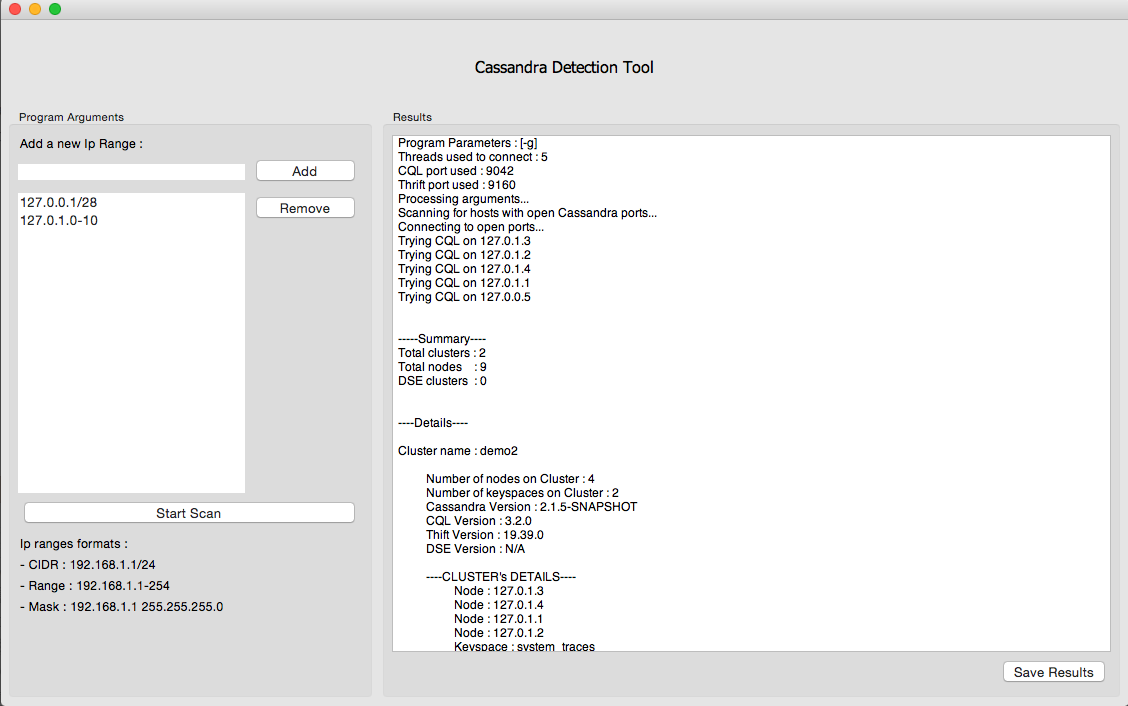
\includegraphics[scale=0.37]{cdt-preview.png}
\caption{Cassandra Detection Tool}
\label{fig:cdt}
\end{figure}

\section{Additional work}
After building the product and made basic optimizations and tests on it, I had the goal to make it compatible on multiple platforms (e.g. CLI and GUI are fully working on \emph{Linux}, \emph{Mac OS} and \emph{Windows}). For the core application it was not a problem because it was written in Java. Whereas other external tools like \emph{nmap} written in C++, and \emph{Eclipse Swift} were both natively not portable, and required specific compiled versions for achitectures and OS. They required a bit of work to make functional executables. It was also required to build an Installer for the application that had to be the most simple possible, I did that using \emph{InstallBuilder}\footnote{Had some complications on this part with for example \emph{nmap} on \emph{Windows}, that requires the installation of WinPcap, so this needed to be added transparently in the installation process}. I also added automatically generated native platforms launchers for the program on the GUI interface (i.e. a clickable shortcut on the Desktop after installation). Generating all that additional work and elements have been automated with the building process, using \emph{Maven}, that compiles, packages the application and external tools like nmap, and creates installers, in one \emph{Maven} command.\\
I also worked on making some performance improvements in the code, and did some real situation tests on our test bed in California, with our test bed containing several clusters of hundreds of nodes. The results were quite satisfying, and thanks to nmap we were able to make scans of a CIDR /16 (Class B - 65,536 IP addresses) sub-network in approximately 2 minutes.

\section{Conclusion}
This project offered the opportunity to build this entire application on my own, and have a rather big project to build from scratch. It also gave me the opportunity to make presentations and speeches during company-wide meetings.


\chapter{DSE Graph integration for the Java Driver}
This last topic have been assigned to me 1 month and a half before the end of the internship and I worked almost exclusively on it until the end of the internship.\\
For the first part of this assignment, I have been studying and testing actual Graph databases technologies, in order to understand the requirements of the project. I then wrote a \emph{Design Document} that will help adapting the same API for the solution on all other \ds{} drivers. The final goal was to build a functional prototype of the project.

\section{TinkerPop, TitanDB and DSE Graph}
In this paragraph I will try to bring a bit of technical background necessary to understand the goal of the project I've been working on, explaining the concept of Graph databases, it's open source standard \emph{TinkerPop}, the open source production-oriented version \tdb{}, and the upcoming \ds{} solution, \dseg{}.\\
Graph databases are the new evolution of big data processing solutions, supposed to provide much faster processing and more coverage and simplicity for data analytics in highly connected data sets like Social Networks.\\
The concept is to abstract the view of the real data, under the form of \emph{graphs}, composed of \emph{edges} and \emph{vertices}, and abstracting the backend storage solution running behind the graph engine. Having a graph abstraction of the data, allows usage of complex graph algorithms well known in \emph{Graph theory}, and also opens tons of new possibility of algorithms, for improved data processing.\\
\emph{Gremlin}, as a graph traversal language, is a functional language implemented in the user's native programming language and is used to define the $\Psi$ of a Gremlin machine.\\
The data is represented in \emph{Gremlin} as a graph $G$, where $G = (V, E, \lambda)$, and $V$ is a set of vertices, $E$ is a multiset of directed binary edges, and $\lambda$ is a partial function that maps an element/string pair to an object in the universal set $U$ (excluding vertices and edges as allowed property values).\\
We also define a traversal $\Psi$, and a set of traversers $T$, where the traversers move about the graph according to the instructions specified in the traversal, where the result of the computation is the ultimate locations of all halted traversers. The graph algorithm will then be the instructions included in $\Psi$ and will start from a set of vertices restrained initially and run through the graph, going from a vertex to another through the edges, if the destination vertex meets the requirements of the current step in $\Psi$.\\
\tp{} is a computing framework providing different Java implementations of Graph computing engines and offers a ready-to-use solution to easily setting up a Graph database solution, it is considered as the open source standard for Graph databases, and its architecture allows any Vendor to plug its implementation of graphs and traversals easily. Therefore, we reference graph computing implemented on top of \emph{Hadoop}, \emph{Spark}\footnote{With \emph{SparkGraphComputer} for example, the graph is distributed with the Hadoop input format and message passing is coordinated via Spark map/reduce/join operations on in-memory and disk-cached data. So it is possible to add operations from the \emph{Spark} library after the processing of a traversal, to build classic \emph{Spark} analytics over the graph traversal results.}, \emph{Neo4j}, or an in-memory implementation also exists named \emph{TinkerGraph}.\\
\begin{lstlisting}[label=grml-ex-1, caption=Quick example of the syntax of Gremlin on a simple Traversal executed in the Gremlin-Console (from TinkerPop) in the Groovy language, style=Java]

gremlin> graph = TinkerFactory.createModern()
==>tinkergraph[vertices:6 edges:6]
gremlin> g = graph.traversal(standard())
==>graphtraversalsource[tinkergraph[vertices:6 edges:6], standard]
gremlin> g.V().has('name','marko').out('knows').values('name')
==>vadas
==>josh
\end{lstlisting}
This example shows how to get all the Vertices names that the Vertex with the property \verb;"name":"marko"; has on outgoing edges with the property \verb;"knows";.\\
\tdb{} is also an open-source implementation of \emph{Gremlin}'s graph computing engine, providing highly tested and powerful Graph implementation with the option of multiple back-end environments such as \emph{BerkeleyDB}, \emph{Apache HBase}, or \ca{}. It also supports indexing backends like \emph{Solr}, \emph{ElasticSearch} or \emph{Apache Lucene}. \tdb{} has been created and is maintained by the originators of \tp{} and \emph{Gremlin}, known as the company \emph{Aurelius}.\\
\emph{Aurelius} have been recently bought by \ds{}, for the final goal of the creation of \emph{DSE Graph}. \dseg{} is destined to be, as \emph{DataStax Enterprise} is for \ca{}, the production-ready, supported and optimized next version of \tdb{}, only running on and fully optimized for \emph{DataStax Enterprise}, which means \ca{}, and \emph{Solr}.

\section{What does that mean for the DataStax Java Driver}
\emph{DSE Graph}'s engine integrated to \emph{DataStax Enterprise} (or \emph{DSE}) will bring a whole new set of possibilities, all conveniently configured within usual \emph{DSE} instances. However, these functionalities have to be accessible to users, so \emph{DataStax} Drivers need to sync with these new \dseg{} features.\\
The purpose of this adaptation is to first make the driver able to send Gremlin requests that the \dseg{} server would be able to intercept and differentiate from a \emph{CQL} query. Then the \dseg{} server would take care of processing the result, and send the result to the driver. Therefore, the driver needs to provide a meaningful API to allow users to interact efficiently with the server and process the results.

\section{Technical challenges}
The technical difficulty to achieve this integration, is to make the \djd{} able to \underline{handle the dynamic nature of the \emph{Gremlin} language}. From the driver's point of view, a statement is considered as a basic String containing a query, that is encoded in a \verb;ByteBuffer; and sent through the \emph{Native protocol}, then this is not considered to be a major show-stopper for the compatibility. However, when any result from a \emph{CQL} query is sent through the \emph{Native protocol} to be interpreted on the driver, this results contains metadata that are crucial to decode the types and content of the data in the response. It is not that simple with \emph{Gremlin}. Basically the return type of a result can be determined during the traversal, and can change during it. It is then not possible to determine afore the type of a result and it is not possible to encode the data returned with the usual \emph{CQL} data types. This kind of specificity prevents the drivers from natively supporting \dseg{}, and \emph{Gremlin}. In other words, \emph{Gremlin} needs to be able to return schemaless results, meaning that the result types are not known until the result is realized as part of query execution and result iteration. The basic approach for satisfying the above requirements is to \underline{embed a subprotocol within the Cassandra protocol}. At the most simple level, the subprotocol will be implemented by using \emph{blob fields} within requests and responses.\\
Finally, it has been decided that the content of these \emph{blob} fields would be encoded in \emph{JSON}, using \tp{}'s \emph{GraphSON} library.





\begin{thebibliography}{99}
  \bibitem[1]{Lamport1} Leslie Lamport.
  	\newblock \textit{Paxos Made Simple.}
  	\newblock ACM SIGACT News (Distributed Computing Column), 2001.

  \bibitem[2]{Google1} Tushar Chandra, Robert Griesemer, Joshua Redstone.
  	\newblock \textit{Paxos Made Live - An Engineering Perspective.}
  	\newblock June 20, 2007.

  \bibitem[3]{Aniello13} Leonardo Aniello, Silvia Bonomi, Marta Breno, Roberto Baldoni.
    \newblock \textit{Assessing Data Availability of Cassandra in the Presence
of non-accurate Membership.}
	\newblock University of Rome, Italy, 2013.
  
  \bibitem[4]{Martin} Jean-Philippe Martin, Lorenzo Alvisi.
    \newblock \textit{Fast Byzantine Paxos}.

\end{thebibliography}



\end{document}

















































